\documentclass[12pt,a4paper]{article}
\usepackage[utf8]{inputenc}
\usepackage{amsmath}
\usepackage{amsfonts}
\usepackage{amssymb}
\usepackage[none]{hyphenat}
\usepackage{enumerate}
\usepackage[spanish]{babel}
\usepackage{graphicx}
\usepackage{float}
\usepackage{array}
\usepackage{listings}
\usepackage{tcolorbox}
\graphicspath{ {IMAGES/} }
\pagestyle{headings}
\author{Juan Sebastian Gonzalez Camacho (1968220), Andrés Felipe Ruíz Buriticá (1968171), Jhoan Sebastian Rojas Holguin (1958337), Carlos Alberto Delgado Galeano (1968127), Jesus Alberto Gil Ayala (1968231)}
\title{Borvo MO - Requirements Specification}
\begin{document}
\begin{titlepage}
\centering
{
\includegraphics[width=0.18 \textwidth]{logo.png} \par}
\vfill
{\bfseries\LARGE Universidad del Valle\par}
{\Large Sede Tuluá\par}
\vfill
{\scshape\Large Ingeniería de Sistemas \par}
\vfill
{\scshape\Huge Borvo - Medicinae Operam \par}
\vfill
{\itshape\Large Avance 1 - Proyecto Final de Bases de Datos y Desarrollo de Software I \par}
\vfill
{\Large Autores: \par}
{\Large Andrés Felipe Ruíz Buriticá - 1968171 \par}
{\Large Carlos Alberto Delgado Galeano - 1968127 \par}
{\Large Jesús Alberto Gil Ayala - 1968231 \par}
{\Large Jhoan Sebastian Rojas Holguin - 1958337 \par}
{\Large Juan Sebastian González Camacho - 1968220 \par}
\vfill
{\Large 11 de Noviembre del 2022 \par}
\end{titlepage}
\tableofcontents
\newpage
\section{Requisitos Específicos}
\subsection{Requisitos Funcionales}
\newcounter{RF}
\begin{center}
\begin{tabular}{|m{5.5cm}|m{9.5cm}|}
\hline
\textbf{Identificador} & RF-\stepcounter{RF}\arabic{RF}\\
\hline
\textbf{Nombre} & Gestionar afiliados cotizantes de la EPS.\\
\hline
\textbf{Descripción} & El sistema debe permitir gestionar toda la información de los cotizantes de la EPS: Tipo de documento, número de documento de identidad, apellidos, nombres, fecha de nacimiento, género, dirección, ciudad de residencia, teléfono, estado civil, correo electrónico, fecha de la primera afiliación, estado actual (Activo, Inactivo, Retirado), salario, rango salarial. La gestión de esta información está constituida por 4 subrequisitos funcionales:
\begin{itemize}
\item RF-01.1: Registrar cotizante.
\item RF-01.2: Consultar cotizante.
\item RF-01.3: Modificar cotizante.
\item RF-01.4: Eliminar cotizante.
\end{itemize}\\
\hline
\textbf{Prioridad} & Alta.\\
\hline
\end{tabular}
\vspace{5mm}

\begin{tabular}{|m{5.5cm}|m{9.5cm}|}
\hline
\textbf{Identificador} & RF-\stepcounter{RF}\arabic{RF}\\
\hline
\textbf{Nombre} & Gestionar los beneficiarios que tiene cada cotizante.\\
\hline
\textbf{Descripción} & El sistema debe permitir gestionar la información de los  beneficiarios que puede tener cada cotizante: Tipo y número de documento de identidad, apellidos, nombres, fecha de nacimiento, género, dirección, ciudad de residencia, teléfono, estado civil, correo electrónico y parentesco con el cotizante y estado actual. La gestión de esta información está constituida por 4 subrequisitos funcionales:
\begin{itemize}
\item RF-02.1: Registrar beneficiario.
\item RF-02.2: Consultar beneficiario.
\item RF-02.3: Modificar beneficiario.
\item RF-02.4: Eliminar beneficiario.
\end{itemize}\\
\hline
\textbf{Prioridad} & Alta.\\
\hline
\end{tabular}
\vspace{5mm}

\begin{tabular}{|m{5.5cm}|m{9.5cm}|}
\hline
\textbf{Identificador} & RF-\stepcounter{RF}\arabic{RF}\\
\hline
\textbf{Nombre} & Gestionar las empresas que contratan a los cotizantes.\\
\hline
\textbf{Descripción} & El sistema debe permitir gestionar la información de las empresas que contratan a los cotizantes dependientes: Nit, razón social, ciudad, dirección, teléfono, nombre del contacto. En el caso de los trabajadores independientes se debe registrar el mismo cotizante como empresa, registrando el RUT en lugar del Nit y se crea un contrato. La gestión de esta información está constituida en 4 subrequisitos funcionales:
\begin{itemize}
\item RF-03.1: Registrar empresa.
\item RF-03.2: Consultar empresa.
\item RF-03.3: Modificar empresa.
\item RF-03.4: Eliminar empresa.
\end{itemize}\\
\hline
\textbf{Prioridad} & Alta.\\
\hline
\end{tabular}
\vspace{5mm}

\begin{tabular}{|m{5.5cm}|m{9.5cm}|}
\hline
\textbf{Identificador} & RF-\stepcounter{RF}\arabic{RF}\\
\hline
\textbf{Nombre} & Gestionar las IPS que prestan los servicios a sus afiliados.\\
\hline
\textbf{Descripción} & El sistema debe permitir gestionar la información de las IPS que están contratadas por la EPS: Nit, razón social, nivel de atención, servicios que presta. La gestión de esta información está dividida en 4 subrequisitos funcionales:
\begin{itemize}
\item RF-04.1: Registrar IPS.
\item RF-04.2: Consultar IPS.
\item RF-04.3: Modificar IPS.
\item RF-04.4: Eliminar IPS.
\end{itemize}\\
\hline
\textbf{Prioridad} & Alta.\\
\hline
\end{tabular}
\vspace{5mm}

\begin{tabular}{|m{5.5cm}|m{9.5cm}|}
\hline
\textbf{Identificador} & RF-\stepcounter{RF}\arabic{RF}\\
\hline
\textbf{Nombre} & Gestionar órdenes de servicio.\\
\hline
\textbf{Descripción} & El sistema debe permitir gestionar la información de las órdenes de servicio que llevan los afiliados a la EPS, que les entrega la IPS en donde fueron atendidos: Código y fecha de la orden, nombre del médico que la formula, diagnóstico, descripción de los servicios formulados. La gestión de esta información se divide en 2 subrequisitos funcionales:
\begin{itemize}
\item RF-05.1: Registrar órden.
\item RF-05.2: Consultar órden.
\end{itemize}\\
\hline
\textbf{Prioridad} & Alta.\\
\hline
\end{tabular}
\vspace{5mm}

\begin{tabular}{|m{5.5cm}|m{9.5cm}|}
\hline
\textbf{Identificador} & RF-\stepcounter{RF}\arabic{RF}\\
\hline
\textbf{Nombre} & Generar reportes de afiliados.\\
\hline
\textbf{Descripción} & El sistema debe permitir generar los siguientes reportes de los afiliados:
\begin{itemize}
\item RF-06.1: Listado de afiliados por estado.
\item RF-06.2: Listado de afiliados activos de una IPS.
\item RF-06.3: Listado de afiliados inactivos.
\item RF-06.4: Listado de afiliados independientes organizados por estado.
\end{itemize}\\
\hline
\textbf{Prioridad} & Alta.\\
\hline
\end{tabular}
\vspace{5mm}

\begin{tabular}{|m{5.5cm}|m{9.5cm}|}
\hline
\textbf{Identificador} & RF-\stepcounter{RF}\arabic{RF}\\
\hline
\textbf{Nombre} & Generar reportes de órdenes de servicio.\\
\hline
\textbf{Descripción} & El sistema debe permitir generar un reporte de todas las órdenes de servicio por paciente.\\
\hline
\textbf{Prioridad} & Alta.\\
\hline
\end{tabular}
\vspace{5mm}

\begin{tabular}{|m{5.5cm}|m{9.5cm}|}
\hline
\textbf{Identificador} & RF-\stepcounter{RF}\arabic{RF}\\
\hline
\textbf{Nombre} & Reportar pago de aportes.\\
\hline
\textbf{Descripción} & El sistema debe permitir al banco reportar mensualmente el pago de aportes de cada empleado con contrato activo, este reporte debe incluir la fecha de pago, el valor pagado, la información del cotizante y la información de la empresa que hace el pago. Los trabajadores independientes también deben reportar mensualmente su pago de aportes. Este se puede hacer individual o en bloque de archivos.\\
\hline
\textbf{Prioridad} & Alta.\\
\hline
\end{tabular}
\vspace{5mm}

\begin{tabular}{|m{5.5cm}|m{9.5cm}|}
\hline
\textbf{Identificador} & RF-\stepcounter{RF}\arabic{RF}\\
\hline
\textbf{Nombre} & El cotizante puede consultar su propia información.\\
\hline
\textbf{Descripción} & El sistema debe permitir a cada cotizante consultar su propia información.\\
\hline
\textbf{Prioridad} & Media.\\
\hline
\end{tabular}
\vspace{5mm}

\begin{tabular}{|m{5.5cm}|m{9.5cm}|}
\hline
\textbf{Identificador} & RF-\stepcounter{RF}\arabic{RF}\\
\hline
\textbf{Nombre} & Generar listado de pago de aportes.\\
\hline
\textbf{Descripción} & El sistema debe permitir generar un listado de los aportes recibidos por un afiliado en un período de tiempo determinado.\\
\hline
\textbf{Prioridad} & Media.\\
\hline
\end{tabular}
\vspace{5mm}

\begin{tabular}{|m{5.5cm}|m{9.5cm}|}
\hline
\textbf{Identificador} & RF-\stepcounter{RF}\arabic{RF}\\
\hline
\textbf{Nombre} & Generar listado de citas.\\
\hline
\textbf{Descripción} & El sistema debe permitir generar un listado de citas en una fecha e IPS en particular.\\
\hline
\textbf{Prioridad} & Media.\\
\hline
\end{tabular}
\vspace{5mm}
\end{center}
\subsection{Requisitos No Funcionales}
\newcounter{RNF}
\begin{center}
\begin{tabular}{|m{5.5cm}|m{9.5cm}|}
\hline
\textbf{Identificador} & RNF-\stepcounter{RNF}\arabic{RNF}\\
\hline
\textbf{Nombre} & Diseño de interfaz amigable.\\
\hline
\textbf{Descripción} & El software debe ser sencillo e intuitivo para una mejor comprensión de los usuarios.\\
\hline
\textbf{Categoría} & Usabilidad.\\
\hline
\end{tabular}
\vspace{5mm}

\begin{tabular}{|m{5.5cm}|m{9.5cm}|}
\hline
\textbf{Identificador} & RNF-\stepcounter{RNF}\arabic{RNF}\\
\hline
\textbf{Nombre} & Software ágil.\\
\hline
\textbf{Descripción} & El software debe generar la información y mostrar formularios y guías claros y concisos.\\
\hline
\textbf{Categoría} & Usabilidad.\\
\hline
\end{tabular}
\vspace{5mm}

\begin{tabular}{|m{5.5cm}|m{9.5cm}|}
\hline
\textbf{Identificador} & RNF-\stepcounter{RNF}\arabic{RNF}\\
\hline
\textbf{Nombre} & Disponible.\\
\hline
\textbf{Descripción} & El software estará en funcionamiento todo el tiempo.\\
\hline
\textbf{Categoría} & Desempeño.\\
\hline
\end{tabular}
\vspace{5mm}

\begin{tabular}{|m{5.5cm}|m{9.5cm}|}
\hline
\textbf{Identificador} & RNF-\stepcounter{RNF}\arabic{RNF}\\
\hline
\textbf{Nombre} & Tolerante al error.\\
\hline
\textbf{Descripción} & El sistema proveerá información con respecto al error en la ejecución de alguna función y añadirá una recomendación.\\
\hline
\textbf{Categoría} & Desempeño.\\
\hline
\end{tabular}
\vspace{5mm}

\begin{tabular}{|m{5.5cm}|m{9.5cm}|}
\hline
\textbf{Identificador} & RNF-\stepcounter{RNF}\arabic{RNF}\\
\hline
\textbf{Nombre} & Permisos de usuario.\\
\hline
\textbf{Descripción} & El sistema solicitará usuario y contraseña para determinar los permisos según el perfil de usuario.\\
\hline
\textbf{Categoría} & Seguridad.\\
\hline
\end{tabular}
\vspace{5mm}

\begin{tabular}{|m{5.5cm}|m{9.5cm}|}
\hline
\textbf{Identificador} & RNF-\stepcounter{RNF}\arabic{RNF}\\
\hline
\textbf{Nombre} & Personal autorizado.\\
\hline
\textbf{Descripción} & Al sistema solo pueden ingresar los usuarios autorizados que están registrados en la base de datos.\\
\hline
\textbf{Categoría} & Seguridad.\\
\hline
\end{tabular}
\vspace{5mm}

\begin{tabular}{|m{5.5cm}|m{9.5cm}|}
\hline
\textbf{Identificador} & RNF-\stepcounter{RNF}\arabic{RNF}\\
\hline
\textbf{Nombre} & Tiempo de respuesta\\
\hline
\textbf{Descripción} & El sistema debe enviar una respuesta en el acceso y uso de sus funciones en no más de 10 segundos.\\
\hline
\textbf{Categoría} & Eficiencia.\\
\hline
\end{tabular}
\vspace{5mm}

\begin{tabular}{|m{5.5cm}|m{9.5cm}|}
\hline
\textbf{Identificador} & RNF-\stepcounter{RNF}\arabic{RNF}\\
\hline
\textbf{Nombre} & Acceso desde varios dispositivos.\\
\hline
\textbf{Descripción} & El sistema debe ser un aplicativo web que permita ingresar desde cualquier dispositivo.\\
\hline
\textbf{Categoría} & Portabilidad.\\
\hline
\end{tabular}
\vspace{5mm}
\end{center}
\section{Aspectos de Diseño}
\subsection{Modelo Entidad Relación}
\begin{figure}[H]
\centering
{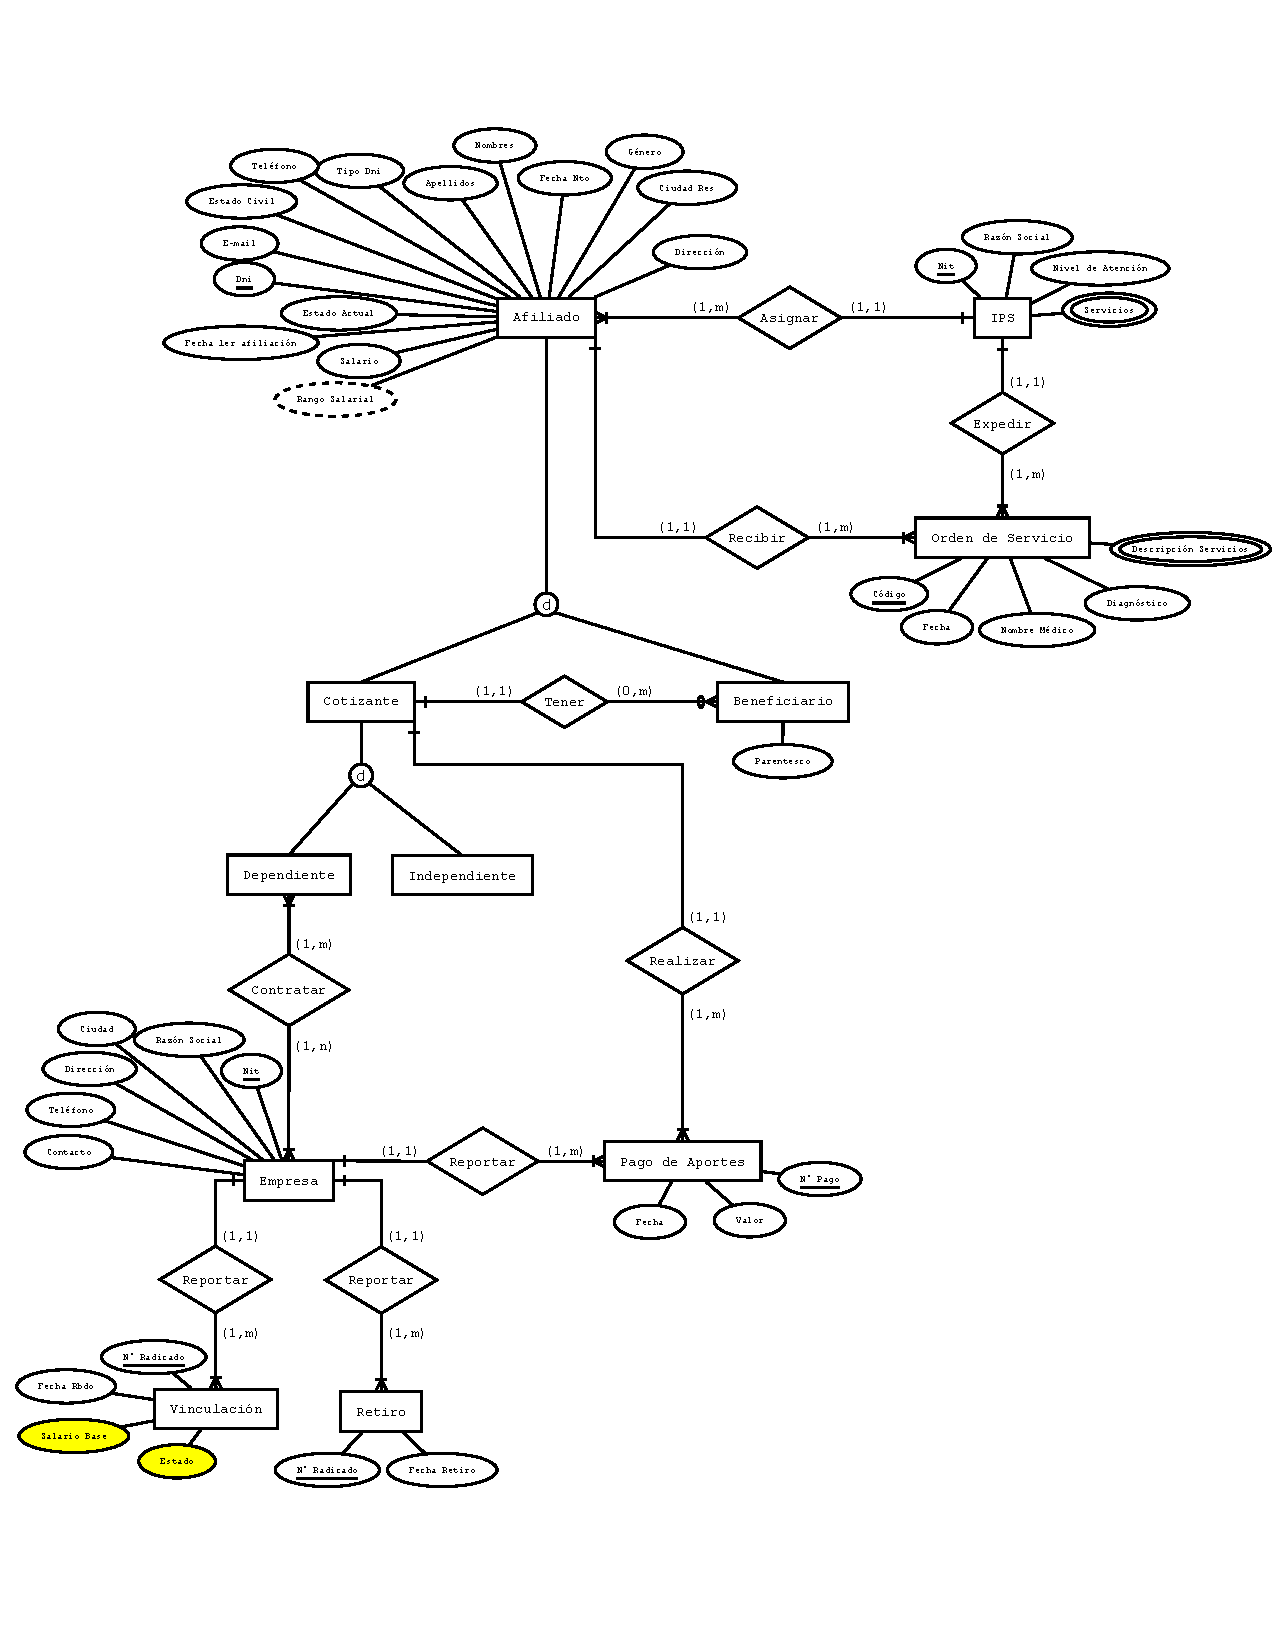
\includegraphics[width=1\textwidth]{Entity_relationship_diagram.pdf} \par}
\caption{Modelo Entidad - Relación.}
\end{figure}
\subsection{Modelo Relacional}
\begin{tcolorbox}[title=Modelo Relacional]
\textbf{AFILIADO} (\underline{Dni}, TipoDi, Apellidos, Nombres, FechaNto, Género, Dirección, CiudadResidencia, Teléfono, EstadoCivil, EMail, EstadoActual, IPS)
\begin{itemize}
\item IPS $\rightarrow$ IPS.Nit
\end{itemize}
\textbf{COTIZANTE} (\underline{Dni}, TipoCotizante, FechaPrimerAfiliación, Salario, RangoSalarial)
\begin{itemize}
\item Dni $\rightarrow$ AFILIADO.Dni
\end{itemize}
\textbf{BENEFICIARIO} (\underline{Dni}, Parentesco, Cotizante)
\begin{itemize}
\item Dni $\rightarrow$ AFILIADO.Dni
\item Cotizante $\rightarrow$ COTIZANTE.Dni
\end{itemize}
\textbf{CONTRATAR} (\underline{Cotizante}, \underline{Empresa})
\begin{itemize}
\item Cotizante $\rightarrow$ COTIZANTE.Dni
\item Empresa $\rightarrow$ EMPRESA.Nit
\end{itemize}
\textbf{EMPRESA} (\underline{Nit}, RazónSocial, Ciudad, Dirección, Teléfono, NombreContacto)\\

\textbf{VINCULACIÓN} (\underline{N°Radicado}, FechaRecibido, Empresa, Cotizante)
\begin{itemize}
\item Empresa $\rightarrow$ EMPRESA.Nit
\item Cotizante $\rightarrow$ COTIZANTE.Dni
\end{itemize}
\textbf{RETIRO} (\underline{N°Radicado}, FechaRetiro, Empresa, Cotizante)
\begin{itemize}
\item Empresa $\rightarrow$ EMPRESA.Nit
\item Cotizante $\rightarrow$ COTIZANTE.Dni
\end{itemize}
\textbf{PAGO\_APORTES} (\underline{N°Pago}, Fecha, Valor, Empresa, Cotizante)
\begin{itemize}
\item Empresa $\rightarrow$ EMPRESA.Nit
\item Cotizante $\rightarrow$ COTIZANTE.Dni
\end{itemize}
\textbf{IPS} (\underline{Nit}, RazónSocial, NivelAtención)\\

\textbf{SERVICIOS} (\underline{IPS}, \underline{Servicio})
\begin{itemize}
\item IPS $\rightarrow$ IPS.Nit
\end{itemize}
\end{tcolorbox}
\begin{tcolorbox}
\textbf{ORDEN\_SERVICIO} (\underline{Código}, Fecha, NombreMédico, Diagnóstico, IPS, Afiliado)
\begin{itemize}
\item IPS $\rightarrow$ IPS.Nit
\item Afiliado $\rightarrow$ AFILIADO.Dni
\end{itemize}
\textbf{DESCRIPCIÓN\_SERVICIOS} (\underline{Orden}, \underline{DescripciónServicio})
\begin{itemize}
\item Orden $\rightarrow$ ORDEN\_SERVICIO.Código
\end{itemize}
\end{tcolorbox}
\subsection{Instrucciones SQL}
\begin{tcolorbox}[title=Insertar afiliado]
\textbf{insert} \textbf{into} afiliado \textbf{values} (`5678',`Cedula', `Gil Ayala', `Chucho',
 `2-22-1999', `Masculino', `Calle 61 \# 122', 'Cali', `2263322', `Casado',
 `chuchogil@gmail', `Activo', `83500012')
\end{tcolorbox}
\begin{tcolorbox}[title=Insertar empresa]
\textbf{insert} \textbf{into} empresa \textbf{values} (`010203',`Colombina S.A',`La Paila',`Zarzal',`6022339200',`Colombina')
\end{tcolorbox}
\begin{tcolorbox}[title=Insertar pago de aportes]
\textbf{insert} \textbf{into} pago\_aportes \textbf{values} (`01', `1-01-2022', `120000', `010203', `12345')
\end{tcolorbox}
\begin{tcolorbox}[title=Insertar vinculación]
\textbf{insert} \textbf{into} vinculacion \textbf{values} (`01', `2022-11-11', `4552000', `342221')
\end{tcolorbox}
\begin{tcolorbox}[title=Insertar retiro]
\textbf{insert} \textbf{into} retiro \textbf{values} (`01', `2022-11-11', `4552000', `342221')
\end{tcolorbox}
\begin{tcolorbox}[title=Listado de afiliados activos de una IPS]
\textbf{select} nombres, apellidos\\
\textbf{from} afiliado\\
\textbf{where} IPS = `123456' \textbf{and} estadoactual = `Activo'
\end{tcolorbox}
\begin{tcolorbox}[title=Listado de afiliados inactivos]
\textbf{select} nombres, apellidos\\
\textbf{from} afiliado\\
\textbf{where} estadoactual = `Inactivo'
\end{tcolorbox}
\begin{tcolorbox}[title=Listado de aportes recibidos por un afiliado en un periodo de tiempo]
\textbf{select} *\\
\textbf{from} pago\_aportes\\
\textbf{where} cotizante = `123456' \textbf{and} fecha \textbf{between} `AAAA-MM-DD' \textbf{and} `AAAA-MM-DD'
\end{tcolorbox}
\begin{tcolorbox}[title=Listado de citas en una IPS y fecha particular]
\textbf{select} *\\
\textbf{from} orden\_de\_servicio\\
\textbf{where} IPS = `123456' \textbf{and} fecha = `AAAA-MM-DD'
\end{tcolorbox}
\begin{tcolorbox}[title=Listado de afiliados independientes organizados por estado]
\textbf{select} * \\
\textbf{from} afiliado\\ 
\textbf{where} DNI \textbf{in}\\
		(\textbf{select} DNI\\
		\textbf{from} cotizante\\
		\textbf{where} tipocotizante = 'dependiente')\\
		\textbf{order by} estadoactual
\end{tcolorbox}
\end{document}